% The generic preamble
\documentclass[10pt,letterpaper,fleqn,titlepage]{article}

% Define packages to use
\usepackage{natbib}
\usepackage[dvips]{graphicx,color}
\usepackage{amsmath,amssymb}
\usepackage{bm}
\usepackage{caption}
\usepackage{xr}
\usepackage{ifthen}
\usepackage[dvipdfm,colorlinks,linkcolor=blue,citecolor=blue,urlcolor=blue]{hyperref}
\usepackage{fancybox}
\usepackage{textcomp}
\usepackage{alltt}
%\usepackage{floatflt}
%\usepackage{svn}


% Redefine default page
\setlength{\textheight}{9in}  % 1" above and below
\setlength{\textwidth}{6.75in}   % 0.5" left and right
\setlength{\oddsidemargin}{-0.25in}

% Redefine default paragraph
\setlength{\parindent}{0pt}
\setlength{\parskip}{1ex plus 0.5ex minus 0.2ex}

% Define caption width and default fonts
\setlength{\captionmargin}{0.5in}
\renewcommand{\captionfont}{\sffamily}
\renewcommand{\captionlabelfont}{\bfseries\sffamily}

% Define commands for super- and subscript in text mode
\newcommand{\superscript}[1]{\ensuremath{^\textrm{#1}}}
\newcommand{\subscript}[1]{\ensuremath{_\textrm{#1}}}

% Derived commands
\newcommand{\invcm}{\textrm{cm\superscript{-1}}}
\newcommand{\micron}{\ensuremath{\mu\textrm{m}}}

\newcommand{\df}{\ensuremath{\delta f}}
\newcommand{\Df}{\ensuremath{\Delta f}}
\newcommand{\dx}{\ensuremath{\delta x}}
\newcommand{\Dx}{\ensuremath{X_{max}}}
\newcommand{\Xeff}{\ensuremath{X_{eff}}}

\newcommand{\water}{\textrm{H\subscript{2}O}}
\newcommand{\carbondioxide}{\textrm{CO\subscript{2}}}
\newcommand{\ozone}{\textrm{O\subscript{3}}}

\newcommand{\taup}[1]{\ensuremath{\tau_{#1}}}
\newcommand{\efftaup}[1]{\ensuremath{\tau_{#1}^{*}}}

\newcommand{\textbfm}[1]{\boldmath\ensuremath{#1}\unboldmath}

\newcommand{\rb}[1]{\raisebox{1.5ex}[0pt]{#1}}

\newcommand{\f}[1]{\texttt{#1}}

% Define how equations are numbered
\numberwithin{equation}{section}
\numberwithin{figure}{section}
\numberwithin{table}{section}

% Define a command for title page author email footnote
\newcommand{\email}[1]
{%
  \renewcommand{\thefootnote}{\alph{footnote}}%
  \footnote{#1}
  \renewcommand{\thefootnote}{\arabic{footnote}}
}

% Define a command to print the Office Note subheading
\newcommand{\notesubheading}[1]
{%
  \ifthenelse{\equal{#1}{}}{}
  { {\Large\bfseries Office Note #1\par}%
    {\scriptsize \sc This is an unreviewed manuscript, primarily intended for informal}\\ 
    {\scriptsize \sc exchange of information among JCSDA researchers\par}%
  }
}

% Redefine the maketitle macro
\makeatletter
\def\docseries#1{\def\@docseries{#1}}
\def\docnumber#1{\def\@docnumber{#1}}
\renewcommand{\maketitle}
{%
  \thispagestyle{empty}
  \vspace*{1in}
  \begin{center}%
     \sffamily
     {\huge\bfseries Joint Center for Satellite Data Assimilation\par}%
     \notesubheading{\@docnumber}
  \end{center}
  \begin{flushleft}%
     \sffamily
     \vspace*{0.5in}
     {\Large\bfseries\ifthenelse{\equal{\@docseries}{}}{}{\@docseries: }\@title\par}%
     \medskip
     {\large\@author\par}%
     \medskip
     {\large\@date\par}%
     \bigskip\hrule\vspace*{2pc}%
  \end{flushleft}%
  \newpage
  \setcounter{footnote}{0}
}
\makeatother
\docseries{}
\docnumber{}


% Define a command for a DRAFT watermark
\usepackage{eso-pic}
\newcommand{\draftwatermark}
{
  \AddToShipoutPicture{%
    \definecolor{lightgray}{gray}{.85}
    \setlength{\unitlength}{1in}
    \put(2.5,3.5){%
      \rotatebox{45}{%
        \resizebox{4in}{1in}{%
          \textsf{\textcolor{lightgray}{DRAFT}}
        }
      }
    }
  }
}





\includeonly{Introduction,Infrared_Channel_SRFs,Radiometric_Impact_of_Interpolation,Impact_of_Wide_Wings,srf.app,bc.app}
% Title info
\title{AVHRR Infrared Spectral Response Function Comparison}
\author{Paul van Delst\email{paul.vandelst@noaa.gov}, David Groff\email{david.groff@noaa.gov}\\JCSDA/EMC/SAIC}
\date{November, 2008}
\docnumber{(unassigned)}
\docseries{CRTM}


%-------------------------------------------------------------------------------
%                            Ze document begins...
%-------------------------------------------------------------------------------
\begin{document}
\maketitle

%\draftwatermark

% The front matter
%=================
\thispagestyle{empty}
\vspace*{10cm}
\begin{center}
  {\sffamily\Large\bfseries Change History}
  \begin{table}[htp]
    \centering
    \begin{tabular}{|p{2cm}|p{3cm}|p{8cm}|}
      \hline
      \sffamily\textbf{Date} & \sffamily\textbf{Author} & \sffamily\textbf{Change}\\
      \hline\hline
      2008-11-01 & P.van Delst & Initial release.\\
      \hline
      2008-11-04 & P.van Delst & Minor corrections from review.\\
      \hline
      2008-11-14 & D.Groff & Added appendice for NOAA-16 cutoff issue.\\
      \hline
      2008-11-18 & P.van Delst & Corrected all references to NOAA-17 SRF difference that were resolved when the correct datafiles were used. Moved NOAA-16 appendix into main document and added additional SRF wing plots.\\
      \hline
      2008-12-16 & D.Groff & Added NOAA-19 data to the radiometric impact and band coefficient tables.\\
      \hline
    \end{tabular}
  \end{table}
\end{center}
\clearpage
\pagenumbering{arabic}
\setcounter{page}{1}


% The main matter
%================
\chapter{Introduction}
%=====================


\section{Components}
%===================
\label{sec:components}

The LBLRTM I/O library is constructed around five data constructs, described in table \ref{tab:component_definitions}:
\begin{table}[htp]
  \centering
  \caption{The data constructs of the LBLRTM I/O library}
  \begin{tabular}{p{2.5cm} p{12cm}}
    \hline\\[-0.1cm]
    \sffamily\textbf{Component Name} & \sffamily\textbf{Description} \\
    \hline\hline\\[-0.2cm]
    \texttt{Fhdr}  & The file header construct that is present at the start of each layer of data. \\\\
    \texttt{Phdr}  & This is the panel header construct that is present at the start of each ``chunk'' of data (usually referred to as a ``panel''. See following.) \\\\
    \texttt{Panel} & This construct corresponds to a ``chunk'' of spectral data. An LBLRTM datafile is referred to as being a single- or double-panel file. The former means a single spectral quantity is present (e.g. optical depth), and the latter means that two spectral quantities are present (e.g. radiance and transmittances). \\\\
    \texttt{Layer} & This construct contains spectral data for the entire frequency range of an LBLRTM calculation for a single layer. The concept ``layer'' can correspond to the spectral data for individual atmospheric layers of the input profile, or to the final result for an entire atmosphere. \\\\
    \texttt{File}  & This contruct is true to its name. It corresponds to an entire datafile of data which may consist of a single layer or multiple layers, and for single- or double-panel spectral data. \\
  \hline
  \end{tabular}
  \label{tab:component_definitions}
\end{table}

Each component has a definition module to define the object and some basic methods to manipulate it, and an I/O module to read and write instances of the objects from/to file.

Two components -- the file header and panel header -- are standalone, but the others contain other components, i.e. the panel object contains panel headers; the layer object contains file headers; and the file object contains layers. A schematic illustration of how the actual LBLRTM datafile format relates to the component definitions is shown in figure \ref{fig:lblrtm_format}.

Note, however, that when an LBLRTM file is read, the individual panel ``chunks'' of spectral data are concatenated into a single spectrum. Thus the \Panel{} object itself is only used when reading from an LBLRTM file and is not used in the \File{} or \Layer{} objects.

\begin{figure}[htp]
  \centering
  \input{graphics/lblrtm_format.pstex_t}
  \caption{Schematic illustration of the LBLRTM single- and double-panel datafile format. A datafile can contain one, or multiple, layers of data.}
  \label{fig:lblrtm_format}
\end{figure}



\section{Conventions}
%====================
\label{sec:conventions}
The following are conventions that have been adhered to in the current release of the LBLRTM I/O library. They are guidelines intended to make understanding the code at a glance easier, to provide a recognisable ``look and feel'', and to minimise name space clashes.



\subsection{Naming of Objects and Instances of Objects}
%------------------------------------------------------

The object\footnote{The terms ``derived type'' and ``structure'' can also be used as the code is not yet fully OO - that's for future updates.} naming convention adopted for use in the LBLRTM I/O library is, 

\hspace{0.4cm}\f{LBLRTM\_}\textit{name}\f{\_type} 

where \textit{name} is an identifier for the particular component (e.g. panel header, layer, file, etc as listed in table \ref{tab:component_definitions}). All object type names are suffixed with ``\f{\_type}''. The ``\f{LBLRTM\_}'' prefix is to define a namespace to minimise name clashes. An instance of a object is then referred to via its \textit{name}, or some sort of derivate of its \textit{name}. Some object declarations examples are,

\begin{alltt}
  TYPE(\hyperref[fig:LBLRTM_File_type_structure]{LBLRTM_File_type}) :: sp_file, dp_file
  TYPE(\hyperref[fig:LBLRTM_Layer_type_structure]{LBLRTM_Layer_type}) :: layer\end{alltt}



\subsection{Naming of Definition Modules}
%----------------------------------------

Modules containing object definitions are termed \textit{definition modules}. These modules contain the actual object definitions as well as various utility procedures that operate on the object. The naming convention adopted for definition modules in the LBLRTM I/O library is, 

\hspace{0.4cm}\f{LBLRTM\_}\textit{name}\f{\_Define} 

where all definition module names are suffixed with ``\f{\_Define}''. The actual source code files for these modules have the same name with a ``\f{.f90}'' suffix.



\subsection{Naming of I/O Modules}
%---------------------------------

Modules containing all the object I/O procedures are termed, surprise, surprise, \textit{I/O modules}. These modules contain function to read and write LBLRTM format datafiles. The naming convention adopted for I/O modules in the LBLRTM I/O library is, 

\hspace{0.4cm}\f{LBLRTM\_}\textit{name}\f{\_IO} 

where all I/O module names are suffixed with ``\f{\_IO}''. As with the definition modules, the actual source code files for these modules have the same name with a ``\f{.f90}'' suffix.



\subsection{Standard Definition Module Procedures}
%-------------------------------------------------

The definition modules for the user-accessible objects (for practical purposes just \File, although \Layer, \Fhdr, \Panel, and \Phdr are accessible for now) contain a standard set of procedures for use with the object being defined. The naming convention for these procedures is,

\hspace{0.4cm}\f{LBLRTM\_}\textit{name}\f{\_}\textit{action}

where the available default actions for each procedure are listed in table \ref{tab:definition_module_default_procedures}. This is not an exhaustive list but procedures for the actions listed in table \ref{tab:definition_module_default_procedures} are generally going to be present.

The exception is that the objects with no allocatable components do not have a creation procedure.

\begin{table}[htp]
  \centering
  \caption{Default action procedures available in object definition modules. $^{\dagger}$Procedures not available for the \Fhdr{} and \Phdr{} objects. $^{\ddagger}$Procedure available only for the \Layer{} object.}
  \begin{tabular}{p{2.5cm} p{3.5cm} p{8.5cm}}
    \hline\\[-0.1cm]
    \sffamily\textbf{Action} & \sffamily\textbf{Type} & \sffamily\textbf{Description} \\
    \hline\hline\\[-0.2cm]
    \texttt{OPERATOR(==)}             & Elemental function   & Tests the equality of two structures. \\
    \texttt{OPERATOR(/=)}             & Elemental function   & Tests the inequality of two structures. \\
    \texttt{Associated}$^{\dagger}$   & Elemental function   & Tests if the object components have been allocated. \\
    \texttt{Create}$^{\dagger}$       & Elemental subroutine & Allocates any allocatable object components. \\
    \texttt{Destroy}                  & Elemental subroutine & Reinitialises an object. \\
    \texttt{DefineVersion}            & Subroutine           & Returns the module version information. \\
    \texttt{Frequency}$^{\ddagger}$   & Subroutine           & Compute and return the spectral frequency grid. \\
    \texttt{Inspect}                  & Subroutine           & Displays object contents to \texttt{stdout}. \\
    \texttt{IsValid}                  & Elemental function   & Tests if the object contains valid data. \\
    \texttt{SetValid}                 & Elemental subroutine & Flags the object as containing valid data. \\
  \hline
  \end{tabular}
  \label{tab:definition_module_default_procedures}
\end{table}

\begin{table}[htp]
  \centering
  \caption{Default action procedures available in object I/O modules.}
  \begin{tabular}{p{2.5cm} p{3.5cm} p{8.5cm}}
    \hline\\[-0.1cm]
    \sffamily\textbf{Action} & \sffamily\textbf{Type} & \sffamily\textbf{Description} \\
    \hline\hline\\[-0.2cm]
    \texttt{IOVersion} & Subroutine  & Returns the module version information. \\
    \texttt{Read}      & Function    & Loads an instance of an object with data read from file. \\
    \texttt{Write}     & Function    & Write an instance of an object to file. \\
  \hline
  \end{tabular}
  \label{tab:io_module_default_procedures}
\end{table}

Some examples of these procedure names are,

\begin{alltt}
  \hyperref[sec:LBLRTM_File_Associated_interface]{LBLRTM_File_Associated}
  \hyperref[sec:LBLRTM_File_IsValid_interface]{LBLRTM_File_IsValid}
  \hyperref[sec:LBLRTM_Layer_Destroy_interface]{LBLRTM_Layer_Destroy}
  \hyperref[sec:LBLRTM_Layer_Frequency_interface]{LBLRTM_Layer_Frequency}
  \hyperref[sec:LBLRTM_File_Inspect_interface]{LBLRTM_File_Inspect}\end{alltt}

The relational operators, \f{==} and \f{/=}, are implemented via overloaded \f{Equal} and \f{NotEqual} action procedures respectively, as is shown below for the \File{} structure,

\begin{alltt}
  INTERFACE OPERATOR(==)
    MODULE PROCEDURE LBLRTM_File_Equal
  END INTERFACE OPERATOR(==)

  INTERFACE OPERATOR(/=)
    MODULE PROCEDURE LBLRTM_File_NotEqual
  END INTERFACE OPERATOR(/=)\end{alltt}

For a complete list of the definition and I/O module procedures for use with the available objects, see appendix \ref{app:object_and_interface_definition}.


\section{AVHRR infrared channel SRFs}
%====================================
\subsection{Gross SRF comparison}
%--------------------------------
Plots of the SRF data for AVHRR channels 3B, 4, and 5 for the NOAA-16 to MetOp-A platforms are shown in appendix \ref{app:srf}. SRF plots for NOAA-16 are shown in figure \ref{fig:avhrr3_n16}, NOAA-17 in figure \ref{fig:avhrr3_n17}, NOAA-18 in figure \ref{fig:avhrr3_n18}, and MetOp-A in figure \ref{fig:avhrr3_metop-a} respectively.

In general, at the scales shown, the SRFs shown in appendix \ref{app:srf} agree quite well. It is at higher magnifications of the SRF data that differences become visible.


\subsection{Interpolation differences}
%-------------------------------------
The main source of differences between the SRFs is due to interpolation. For the AVHRR instruments, the channels responses are typically reported as a function of wavelength (\micron). For the CRTM transmittance production process, we require the SRFs to be,
\begin{itemize}
  \item A function of frequency (\invcm).
  \item At a fixed frequency interval. For broadband infrared instruments, the frequency interval used is 0.1\invcm.
  \item Begun on a 0.1\invcm{} boundary such as 840.0, 900.6, etc.
\end{itemize}
As such, interpolation of the original data is required.

Our regular processing takes the original channel responses and interpolates the data using the IDL\footnote{Interactive Data Language; a scripting language that provides various functionalities for data processing and visualisation} \texttt{SPLINE} function with a tension value of 5.0, selected qualitatively. From the online IDL help\footnote{\href{http://www.ittvis.com/portals/0/pdfs/idl/refguide.pdf}{IDL Reference Guide}; for IDL Version 7.0, November 2007 Edition, see pp2346-2347; Note the download file is quite large.}:

\begin{quote}
If [the tension value] is close to 0, (e.g., .01), then effectively there is a cubic spline fit. If [the tension value] is large, (e.g., greater than 10), then the fit will be like a polynomial interpolation.
\end{quote}

The impacts of the interpolation scheme are shown visually in figures \ref{fig:avhrr3_n16.ch3.srf.zoom} and \ref{fig:avhrr3_n16.ch5.srf.zoom} for NOAA-16 AVHRR/3 channels 3 and 5; figures \ref{fig:avhrr3_n17.ch4.srf.zoom} and \ref{fig:avhrr3_n17.ch5.srf.zoom} for NOAA-17 AVHRR/3 channels 4 and 5; figures \ref{fig:avhrr3_n18.ch3.srf.zoom} and \ref{fig:avhrr3_n18.ch4.srf.zoom} for NOAA-18 AVHRR/3 channels 3 and 4; and in figures \ref{fig:avhrr3_metop-a.ch3.srf.zoom} and \ref{fig:avhrr3_metop-a.ch5.srf.zoom} for MetOp-A AVHRR/3 channels 3 and 5. Only two channels from each instrument are shown with the understanding that the third channel exhinbits the same sort of differences.

For both the NOAA-16 and NOAA-17 instruments, the current SRF data was linearly interpolated from a much lower resolution dataset, and subsequent spline interpolations have little effect. The impact of the spline interpolation on the lower resolution official SRF data is clearly evident. Note also that there is a slight vertical extent difference between the current and official SRF data -- this is most likely due to renormalisation of the SRFs.

In the NOAA-18 AVHRR/3 case, the SRF datasets coincide almost exactly. The differences that do remain can be attributed to the number of decimal places to which the original and intermediate data was reported in ASCII datafiles.

The current SRF data used for MetOp-A AVHRR/3 clearly suffers from quantisation of the data in the original ASCII datafile (reported to only three decimal places). This data was supplied directly by ITT \citep{Sullivan_avhrr3_metop-a_srf} and, at the time, was the only data available. The offical SRF data from \citet{NESDIS_AVHRR_SRFs} is listed as being modified on 04/21/2008, but it is not yet known if those modifications addressed the quantisation problem.

\begin{figure}[htp]
  \centering
  \includegraphics[scale=1]{graphics/zoom/avhrr3_n16.ch3.srf.zoom.eps}
  \caption{Zoom of NOAA-16 AVHRR/3 channel 3B SRF comparison. \textbf{(a)} Complete SRFs showing zoom region 1. \textbf{(b)} Magnification of SRF section from (a) showing zoom region 2.  \textbf{(c)} Magnification of SRF section from (b).}
  \label{fig:avhrr3_n16.ch3.srf.zoom}
\end{figure}

\begin{figure}[htp]
  \centering
  \includegraphics[scale=1]{graphics/zoom/avhrr3_n16.ch5.srf.zoom.eps}
  \caption{Zoom of NOAA-16 AVHRR/3 channel 5 SRF comparison. \textbf{(a)} Complete SRFs showing zoom region 1. \textbf{(b)} Magnification of SRF section from (a) showing zoom region 2.  \textbf{(c)} Magnification of SRF section from (b).}
  \label{fig:avhrr3_n16.ch5.srf.zoom}
\end{figure}

\begin{figure}[htp]
  \centering
  \includegraphics[scale=1]{graphics/zoom/avhrr3_n17.ch4.srf.zoom.eps}
  \caption{Zoom of NOAA-17 AVHRR/3 channel 4 SRF comparison. \textbf{(a)} Complete SRFs showing zoom region 1. \textbf{(b)} Magnification of SRF section from (a) showing zoom region 2.  \textbf{(c)} Magnification of SRF section from (b).}
  \label{fig:avhrr3_n17.ch4.srf.zoom}
\end{figure}

\begin{figure}[htp]
  \centering
  \includegraphics[scale=1]{graphics/zoom/avhrr3_n17.ch5.srf.zoom.eps}
  \caption{Zoom of NOAA-17 AVHRR/3 channel 5 SRF comparison. \textbf{(a)} Complete SRFs showing zoom region 1. \textbf{(b)} Magnification of SRF section from (a) showing zoom region 2.  \textbf{(c)} Magnification of SRF section from (b).}
  \label{fig:avhrr3_n17.ch5.srf.zoom}
\end{figure}

\begin{figure}[htp]
  \centering
  \includegraphics[scale=1]{graphics/zoom/avhrr3_n18.ch3.srf.zoom.eps}
  \caption{Zoom of NOAA-18 AVHRR/3 channel 3B SRF comparison. \textbf{(a)} Complete SRFs showing zoom region 1. \textbf{(b)} Magnification of SRF section from (a) showing zoom region 2.  \textbf{(c)} Magnification of SRF section from (b).}
  \label{fig:avhrr3_n18.ch3.srf.zoom}
\end{figure}

\begin{figure}[htp]
  \centering
  \includegraphics[scale=1]{graphics/zoom/avhrr3_n18.ch4.srf.zoom.eps}
  \caption{Zoom of NOAA-18 AVHRR/3 channel 4 SRF comparison. \textbf{(a)} Complete SRFs showing zoom region 1. \textbf{(b)} Magnification of SRF section from (a) showing zoom region 2.  \textbf{(c)} Magnification of SRF section from (b).}
  \label{fig:avhrr3_n18.ch4.srf.zoom}
\end{figure}


\begin{figure}[htp]
  \centering
  \includegraphics[scale=1]{graphics/zoom/avhrr3_metop-a.ch3.srf.zoom.eps}
  \caption{Zoom of MetOp-A AVHRR/3 channel 3B SRF comparison. \textbf{(a)} Complete SRFs showing zoom region 1. \textbf{(b)} Magnification of SRF section from (a) showing zoom region 2.  \textbf{(c)} Magnification of SRF section from (b).}
  \label{fig:avhrr3_metop-a.ch3.srf.zoom}
\end{figure}

\begin{figure}[htp]
  \centering
  \includegraphics[scale=1]{graphics/zoom/avhrr3_metop-a.ch5.srf.zoom.eps}
  \caption{Zoom of MetOp-A AVHRR/3 channel 5 SRF comparison. \textbf{(a)} Complete SRFs showing zoom region 1. \textbf{(b)} Magnification of SRF section from (a) showing zoom region 2.  \textbf{(c)} Magnification of SRF section from (b).}
  \label{fig:avhrr3_metop-a.ch5.srf.zoom}
\end{figure}


\section{Radiometric impact of SRF interpolation}
%================================================
To determine the radiometric impact of the various forms of the SRF (due to different data sources or different interpolation methods), effective temperatures\footnote{See appendix \ref{app:band_correction_coefficients} for a definition of effective temperature.} for each sensor channel were computed for a blackbody temperature of 285K. The result for the spline interpolated SRF with a tension of 5.0 (spline5) was chosen as the reference. Comparisons were then made with results for a linearly interpolated SRF (linear), a spline interpolated SRF with tension of 0.1 (spline0.1), a spline interpolated SRF with tension of 20 (spline20), the original uninterpolated SRF itself (original), and the current SRF used in CRTM processing (current). The temperature residuals for an SRF type, ``x'', are defined as,
\begin{equation}
  \Delta T(\textrm{x}) = T_{eff}(\textrm{spline5}) - T_{eff}(\textrm{x})
\end{equation}
and are shown in table \ref{tab:teff_comparison}. It is apparent that the type of interpolation used on the SRFs has minimal radiometric impact.

The computed central frequencies and band correction coefficients for the NOAA-16, -17, -18, and MetOp-A AVHRR sensors are shown in appendix \ref{app:band_correction_coefficients}.

\begin{table}[htp]
  \centering
  \begin{tabular}{l c *{6}{r@{.}l}}
    \hline
    \multicolumn{2}{c}{ } & \multicolumn{2}{c}{\textbfm{T_{eff}}} & \multicolumn{2}{c}{\textbfm{\Delta T}} & \multicolumn{2}{c}{\textbfm{\Delta T}} & \multicolumn{2}{c}{\textbfm{\Delta T}} & \multicolumn{2}{c}{\textbfm{\Delta T}} & \multicolumn{2}{c}{\textbfm{\Delta T}} \\
    \textbf{Platform} & \textbf{Channel} & \multicolumn{2}{c}{spline5} & \multicolumn{2}{c}{linear} & \multicolumn{2}{c}{spline0.1} & \multicolumn{2}{c}{spline20} & \multicolumn{2}{c}{original} & \multicolumn{2}{c}{current}\\
    \multicolumn{2}{c}{ } & \multicolumn{2}{c}{(K)} & \multicolumn{2}{c}{(K)} & \multicolumn{2}{c}{(K)} & \multicolumn{2}{c}{(K)} & \multicolumn{2}{c}{(K)}  & \multicolumn{2}{c}{(K)} \\
    \hline\hline
            &  3B & \hspace{0.2em}286&12 & -4&72e-04 &  2&04e-04 & -3&05e-04 &  1&51e-04 &  2&92e-02 \\ 
    NOAA-16 &  4  &               285&01 & -3&43e-06 &  1&73e-06 & -2&28e-06 &  1&76e-06 &  1&26e-05 \\   
            &  5  &               284&98 &  1&08e-05 & -4&00e-06 &  6&84e-06 & -3&62e-06 & -8&87e-05 \vspace{0.75em}\\ 
            &  3B &               286&13 & -4&55e-04 &  1&85e-04 & -2&91e-04 & -1&86e-03 &  6&35e-02 \\   
    NOAA-17 &  4  &               285&01 & -6&02e-06 &  2&70e-06 & -3&92e-06 & -7&89e-05 &  1&35e-03 \\   
            &  5  &               284&98 &  8&72e-06 & -3&24e-06 &  5&52e-06 &  1&60e-04 & -9&14e-04 \vspace{0.75em}\\ 
            &  3B &               286&10 & -4&45e-04 &  1&79e-04 & -2&84e-04 & -3&66e-03 & -3&91e-03 \\   
    NOAA-18 &  4  &               285&01 & -5&17e-06 &  2&29e-06 & -3&36e-06 &  1&15e-05 &  4&70e-06 \\   
            &  5  &               284&98 &  1&09e-05 & -3&91e-06 &  6&89e-06 &  6&55e-06 &  8&00e-06 \vspace{0.75em}\\ 
            &  3B &               286&06 & -4&75e-04 &  1&67e-04 & -2&98e-04 &  1&68e-04 &  0&00e-00 \\   
    NOAA-19 &  4  &               285&01 & -5&11e-06 &  2&24e-06 & -3&32e-06 &  2&25e-06 &  0&00e-00 \\   
            &  5  &               284&98 &  1&08e-05 & -3&90e-06 &  6&78e-06 & -3&56e-06 &  0&00e-00 \vspace{0.75em}\\
            &  3B &               286&33 & -4&28e-04 &  1&82e-04 & -2&75e-04 & -6&51e-03 & -8&11e-03 \\   
    MetOp-A &  4  &               285&01 & -4&68e-06 &  2&15e-06 & -3&06e-06 &  2&98e-06 &  9&08e-07 \\   
            &  5  &               284&98 &  1&17e-05 & -4&24e-06 &  7&43e-06 & -7&09e-06 & -5&24e-06 \\ 
    \hline
  \end{tabular}
  \caption{Effective temperature residuals for a blackbody temperature of 285K between the reference AVHRR SRFs (derived from the NESDIS/STAR AVHRR SRFs \citep{NESDIS_AVHRR_SRFs} via spline interpolation with tension 5.0), different interpolation methods (including none at all), and the current SRF used in CRTM processing.}
  \label{tab:teff_comparison}
\end{table}


\section{Impact of wide SRF wings}
%=================================
To minimise the amount of monochromatic transmittances calculations that are required, the wings of instrument SRFs are truncated. The frequency at which this truncation occurs is somewhat subjective and requires visual inspection of the SRF wings to determine if the data is real, noise, or an artifact of the measurement system. This section is a short description of how this truncation can affect the results when an SRF has wide wings.

Generally, the truncation frequency is selected when the response values decreases below a value of 10\superscript{-4}. In processing the NOAA-16 AVHRR/3 channel 3B data from the \href{http://www.star.nesdis.noaa.gov/smcd/spb/fwu/solar_cal/spec_resp_func}{NESDIS/STAR website}, it was noticed that the shortwave wing of the SRF extended almost two full widths at half-maximum (FWHM) (see the top panel of figure \ref{fig:avhrr3_n16.ch3b.srf}). Close inspection of this shortwave wing revealed that the data was quantised at the 10\superscript{-3} level, and that the wing had a constant value of 0.002 from approximately 2900-3300\invcm{} (see the bottom panel of figure \ref{fig:avhrr3_n16.ch3b.srf}). Because this value is larger than the nominal cutoff magnitude, the entire wing was included in the initial processing.

As shown in figure \ref{fig:avhrr3_n16.ch3b.srf}, frequencies were selected at which to truncate the SRF. The selected $f1$ and $f2$ cutoff frequencies for this channel were 2290\invcm{} and 2920\invcm{}. The impact of this truncation is shown in table \ref{tab:avhrr3_n16.ch3b.srf} where the effective temperatures for a blackbody temperature of 285K differ by 0.13K.

\begin{figure}[htp]
  \centering
  \includegraphics[bb=90 265 540 660,clip,scale=1]{graphics/long_baseline/avhrr3_n16.ch3B.srf.eps}
  \caption{NOAA-16 AVHRR/3 channel 3B SRF indicating the frequencies at which the original SRF data was truncated prior to interpolation. \textbf{(Top panel)} The entire SRF. \textbf{(Bottom panel)} A magnification showing the elevated wings of the SRF.}
  \label{fig:avhrr3_n16.ch3b.srf}
\end{figure}

\begin{table}[htp]
  \centering
  \begin{tabular}{l *{4}{r@{.}l}}
    \hline
                           & \multicolumn{2}{c}{\textbfm{T_{eff}}} & \multicolumn{2}{c}{\textbfm{\nu_o}} & \multicolumn{2}{c}{\textbfm{a_0}} & \multicolumn{2}{c}{\textbfm{a_1}} \\
    \rb{\textbf{SRF Type}} & \multicolumn{2}{c}{(K)}               & \multicolumn{2}{c}{(\invcm)}        & \multicolumn{2}{c}{(K)}           & \multicolumn{2}{c}{(K/K)} \\
    \hline\hline\vspace{-0.5em}\\
    Original (no cutoff)   &   286&25 & 2697&5630 & 2&268358 & 0&996416 \vspace{0.5em}\\ 
    Original (with cutoff) &   286&12 & 2696&4477 & 2&017304 & 0&996841 \vspace{0.5em}\\ 
    \hline
  \end{tabular}
  \caption{Differences in effective temperatures, central frequencies and band correction coefficients for NOAA-16 AVHRR channel 3B due to the reported extended SRF wings. See figure \ref{fig:avhrr3_n16.ch3b.srf}.}
  \label{tab:avhrr3_n16.ch3b.srf}
\end{table}

Given the quantisation of the SRF data for NOAA-16 channel 3B, it is assumed that the wide shortwave wing is a measurement artifact and not a true representation of the SRF response.

While other AVHRR channels (on other platforms) also had wide SRF wings, their wing values were either much closer to zero (e.g., see figures \ref{fig:avhrr3_n17.ch3b.srf} and \ref{fig:avhrr3_n18.ch3b.srf}), or clearly recognisable as measurement noise (e.g. see figure \ref{fig:avhrr3_metop-a.ch5.srf}). However, there are still some SRFs that may require further analysis due the behaviour of their wings (e.g. see figure \ref{fig:avhrr3_n18.ch4.srf}.)

\begin{figure}[htp]
  \centering
  \includegraphics[bb=90 265 540 660,clip,scale=1]{graphics/long_baseline/avhrr3_n17.ch3B.srf.eps}
  \caption{NOAA-17 AVHRR/3 channel 3B SRF indicating the frequencies at which the original SRF data was truncated prior to interpolation. \textbf{(Top panel)} The entire SRF. \textbf{(Bottom panel)} A magnification showing the wings of the SRF.}
  \label{fig:avhrr3_n17.ch3b.srf}
\end{figure}

\begin{figure}[htp]
  \centering
  \includegraphics[bb=90 265 540 660,clip,scale=1]{graphics/long_baseline/avhrr3_n18.ch3B.srf.eps}
  \caption{NOAA-18 AVHRR/3 channel 3B SRF indicating the frequencies at which the original SRF data was truncated prior to interpolation. \textbf{(Top panel)} The entire SRF. \textbf{(Bottom panel)} A magnification showing the wings of the SRF.}
  \label{fig:avhrr3_n18.ch3b.srf}
\end{figure}

\begin{figure}[htp]
  \centering
  \includegraphics[bb=90 265 540 660,clip,scale=1]{graphics/long_baseline/avhrr3_metop-a.ch5.srf.eps}
  \caption{MetOp-A AVHRR/3 channel 5 SRF indicating the frequencies at which the original SRF data was truncated prior to interpolation. \textbf{(Top panel)} The entire SRF. \textbf{(Bottom panel)} A magnification showing the wings of the SRF.}
  \label{fig:avhrr3_metop-a.ch5.srf}
\end{figure}

\begin{figure}[htp]
  \centering
  \includegraphics[bb=90 265 540 660,clip,scale=1]{graphics/long_baseline/avhrr3_n18.ch4.srf.eps}
  \caption{NOAA-18 AVHRR/3 channel 4 SRF indicating the frequencies at which the original SRF data was truncated prior to interpolation. \textbf{(Top panel)} The entire SRF. \textbf{(Bottom panel)} A magnification showing the wings of the SRF.}
  \label{fig:avhrr3_n18.ch4.srf}
\end{figure}


\section{Conclusions}
%====================
Four different ATMS SRFs were used in this study: a simple boxcar SRF derived using the passband widths and frequency offsets; digitised data taken from the ATMS PFM Calibration Data Book\cite{ATMS_PFM_CalLog}, the ``Table 12'' SRFs; digistisations of selected channels from reference \cite{ATMS_PFM_CalLog} performed at SDL, the ``SDL'' SRFs; and digistisations of selected channels from reference \cite{ATMS_PFM_CalLog} performed at NGAS, the ``NGAS'' SRFs.

The degree to which the differences in the SRFs is reflected in the radiative transfer results of section \ref{sec:rt} varies with the channel with no clear pattern.

Comparison of the common SDL and NGAS SRFs indicate that the digitisation process used is not a factor, although the quality of the figures from reference \cite{ATMS_PFM_CalLog} that were used are a factor, as pointed out by both C.L. Chidester and G. DeAmici when they encountered non-orthogonal axes in the scanned figures.

While additional measurements of the NPP ATMS channel responses may no longer be possible, what should be required for future NPOESS ATMS instruments (indeed, \textsl{any} future microwave instrument) is the original digital data of the measured channel responses. This can only serve to mitigate lack of knowledge of the channel spectral response functions as a source of error in the on-orbit measured radiances.



% The references section
%=======================
\clearpage
\bibliographystyle{plainnat}
\bibliography{bibliography}


% The appendices section
%=======================
\begin{appendix}
  \section{ATMS NPP channel SRF comparisons}
%==============================================
\label{app:srf}
This appendix plots the various NPP ATMS microwave spectral response functions (SRFs) used in this study. The "boxcar" data is derived from the data shown in table \ref{tab:atms_fo_sb_and_df}, the "Table 12" data is an edited form of the data from table 12 in reference \cite{ATMS_PFM_CalLog}, and the SDL \cite{ATMS_SRF_SDL} and NGAS \cite{ATMS_SRF_NGAS} data are digitisations of various measured ATMS channel response plots shown in reference \cite{ATMS_PFM_CalLog}.

\clearpage

% Note: the "[H]" placement option is allowed due to the use of the float package
%       in the preamble. I did this to avoid the
%        ! LaTeX Error: Too many unprocessed floats.
%       error due to the large number of figures.

\begin{figure}[H]
  \centering
  \begin{tabular}{c}
    \includegraphics[scale=1]{graphics/srf/atms_npp.ch1.srf.eps} \\
    % the hand-crafted legend
    \setlength{\unitlength}{1cm}
    \begin{picture}(2.0,0.0)(0.0,-2.0)
      \thicklines
      \color{green}
      \put(0.0,0.7 ){\line(1,0){1}}
      \put(1.1,0.55){\sffamily SDL}
      \color{red}
      \put(0.0,1.2 ){\line(1,0){1}}
      \put(1.1,1.05){\sffamily Table 12}
      \color{black}
      \put(0.0,1.7 ){\line(1,0){1}}
      \put(1.1,1.55){\sffamily Boxcar}
    \end{picture} \\\\
    \includegraphics[bb=249 194 1431 1035,scale=0.3]{graphics/log_book/ch1.eps}
  \end{tabular}
  \caption{NPP ATMS channel 1 response. \textbf{(Top)} Boxcar and digitised data. \textbf{(Bottom)} Nominal filter response from ATMS Calibration Data Book\cite{ATMS_PFM_CalLog}.}
  \label{fig:atms_npp.ch1.srf}
\end{figure}

\begin{figure}[H]
  \centering
  \includegraphics[scale=1]{graphics/srf/atms_npp.ch2.srf.eps}
  % the hand-crafted legend
  \setlength{\unitlength}{1cm}
  \begin{picture}(2.0,0.0)(0.0,-2.0)
    \thicklines
    \color{red}
    \put(0.0,1.2 ){\line(1,0){1}}
    \put(1.1,1.05){\sffamily Table 12}
    \color{black}
    \put(0.0,1.7 ){\line(1,0){1}}
    \put(1.1,1.55){\sffamily Boxcar}
  \end{picture}
  \caption{NPP ATMS channel 2 response.}
  \label{fig:atms_npp.ch2.srf}
\end{figure}

\begin{figure}[H]
  \centering
  \includegraphics[scale=1]{graphics/srf/atms_npp.ch3.srf.eps}
  % the hand-crafted legend
  \setlength{\unitlength}{1cm}
  \begin{picture}(2.0,0.0)(0.0,-2.0)
    \thicklines
    \color{red}
    \put(0.0,1.2 ){\line(1,0){1}}
    \put(1.1,1.05){\sffamily Table 12}
    \color{black}
    \put(0.0,1.7 ){\line(1,0){1}}
    \put(1.1,1.55){\sffamily Boxcar}
  \end{picture}
  \caption{NPP ATMS channel 3 response.}
  \label{fig:atms_npp.ch3.srf}
\end{figure}

\begin{figure}[H]
  \centering
  \begin{tabular}{c}
    \includegraphics[scale=1]{graphics/srf/atms_npp.ch4.srf.eps} \\
    % the hand-crafted legend
    \setlength{\unitlength}{1cm}
    \begin{picture}(2.0,0.0)(0.0,-2.0)
      \thicklines
      \color{blue}
      \put(0.0,0.7 ){\line(1,0){1}}
      \put(1.1,0.55){\sffamily NGAS}
      \color{red}
      \put(0.0,1.2 ){\line(1,0){1}}
      \put(1.1,1.05){\sffamily Table 12}
      \color{black}
      \put(0.0,1.7 ){\line(1,0){1}}
      \put(1.1,1.55){\sffamily Boxcar}
    \end{picture} \\\\
    \includegraphics[bb=249 194 1431 1035,scale=0.3]{graphics/log_book/ch4.eps}
  \end{tabular}
  \caption{NPP ATMS channel 4 response. \textbf{(Top)} Boxcar and digitised data. \textbf{(Bottom)} Nominal filter response from ATMS Calibration Data Book\cite{ATMS_PFM_CalLog}.}
  \label{fig:atms_npp.ch4.srf}
\end{figure}

\begin{figure}[H]
  \centering
  \begin{tabular}{c}
    \includegraphics[scale=1]{graphics/srf/atms_npp.ch5.srf.eps} \\
    % the hand-crafted legend
    \setlength{\unitlength}{1cm}
    \begin{picture}(2.0,0.0)(0.0,-2.0)
      \thicklines
      \color{blue}
      \put(0.0,0.7 ){\line(1,0){1}}
      \put(1.1,0.55){\sffamily NGAS}
      \color{red}
      \put(0.0,1.2 ){\line(1,0){1}}
      \put(1.1,1.05){\sffamily Table 12}
      \color{black}
      \put(0.0,1.7 ){\line(1,0){1}}
      \put(1.1,1.55){\sffamily Boxcar}
    \end{picture} \\\\
    \includegraphics[bb=249 194 1431 1035,scale=0.3]{graphics/log_book/ch5.eps}
  \end{tabular}
  \caption{NPP ATMS channel 5 response. \textbf{(Top)} Boxcar and digitised data. \textbf{(Bottom)} Nominal filter response from ATMS Calibration Data Book\cite{ATMS_PFM_CalLog}.}
  \label{fig:atms_npp.ch5.srf}
\end{figure}

\begin{figure}[H]
  \centering
  \includegraphics[scale=1]{graphics/srf/atms_npp.ch6.srf.eps}
  % the hand-crafted legend
  \setlength{\unitlength}{1cm}
  \begin{picture}(2.0,0.0)(3.0,-2.0)
    \thicklines
    \color{red}
    \put(0.0,1.2 ){\line(1,0){1}}
    \put(1.1,1.05){\sffamily Table 12}
    \color{black}
    \put(0.0,1.7 ){\line(1,0){1}}
    \put(1.1,1.55){\sffamily Boxcar}
  \end{picture}
  \caption{NPP ATMS channel 6 response.}
  \label{fig:atms_npp.ch6.srf}
\end{figure}

\begin{figure}[H]
  \centering
  \includegraphics[scale=1]{graphics/srf/atms_npp.ch7.srf.eps}
  % the hand-crafted legend
  \setlength{\unitlength}{1cm}
  \begin{picture}(2.0,0.0)(0.0,-2.0)
    \thicklines
    \color{red}
    \put(0.0,1.2 ){\line(1,0){1}}
    \put(1.1,1.05){\sffamily Table 12}
    \color{black}
    \put(0.0,1.7 ){\line(1,0){1}}
    \put(1.1,1.55){\sffamily Boxcar}
  \end{picture}
  \caption{NPP ATMS channel 7 response.}
  \label{fig:atms_npp.ch7.srf}
\end{figure}

\begin{figure}[H]
  \centering
  \includegraphics[scale=1]{graphics/srf/atms_npp.ch8.srf.eps}
  % the hand-crafted legend
  \setlength{\unitlength}{1cm}
  \begin{picture}(2.0,0.0)(0.0,-2.0)
    \thicklines
    \color{red}
    \put(0.0,1.2 ){\line(1,0){1}}
    \put(1.1,1.05){\sffamily Table 12}
    \color{black}
    \put(0.0,1.7 ){\line(1,0){1}}
    \put(1.1,1.55){\sffamily Boxcar}
  \end{picture}
  \caption{NPP ATMS channel 8 response.}
  \label{fig:atms_npp.ch8.srf}
\end{figure}

\begin{figure}[H]
  \centering
  \begin{tabular}{c}
    \includegraphics[scale=1]{graphics/srf/atms_npp.ch9.srf.eps} \\
    % the hand-crafted legend
    \setlength{\unitlength}{1cm}
    \begin{picture}(2.0,0.0)(0.0,-2.0)
      \thicklines
      \color{blue}
      \put(0.0,0.7 ){\line(1,0){1}}
      \put(1.1,0.55){\sffamily NGAS}
      \color{red}
      \put(0.0,1.2 ){\line(1,0){1}}
      \put(1.1,1.05){\sffamily Table 12}
      \color{black}
      \put(0.0,1.7 ){\line(1,0){1}}
      \put(1.1,1.55){\sffamily Boxcar}
    \end{picture} \\\\
    \includegraphics[bb=249 194 1431 1035,scale=0.3]{graphics/log_book/ch9.eps}
  \end{tabular}
  \caption{NPP ATMS channel 9 response. \textbf{(Top)} Boxcar and digitised data. \textbf{(Bottom)} Nominal filter response from ATMS Calibration Data Book\cite{ATMS_PFM_CalLog}.}
  \label{fig:atms_npp.ch9.srf}
\end{figure}

\begin{figure}[H]
  \centering
  \includegraphics[scale=1]{graphics/srf/atms_npp.ch10.srf.eps}
  % the hand-crafted legend
  \setlength{\unitlength}{1cm}
  \begin{picture}(2.0,0.0)(0.0,-2.0)
    \thicklines
    \color{red}
    \put(0.0,1.2 ){\line(1,0){1}}
    \put(1.1,1.05){\sffamily Table 12}
    \color{black}
    \put(0.0,1.7 ){\line(1,0){1}}
    \put(1.1,1.55){\sffamily Boxcar}
  \end{picture}
  \caption{NPP ATMS channel 10 response.}
  \label{fig:atms_npp.ch10.srf}
\end{figure}

\begin{figure}[H]
  \centering
  \includegraphics[scale=1]{graphics/srf/atms_npp.ch11.srf.eps}
  % the hand-crafted legend
  \setlength{\unitlength}{1cm}
  \begin{picture}(2.0,0.0)(3.5,-2.0)
    \thicklines
    \color{red}
    \put(0.0,1.2 ){\line(1,0){1}}
    \put(1.1,1.05){\sffamily Table 12}
    \color{black}
    \put(0.0,1.7 ){\line(1,0){1}}
    \put(1.1,1.55){\sffamily Boxcar}
  \end{picture}
  \caption{NPP ATMS channel 11 response.}
  \label{fig:atms_npp.ch11.srf}
\end{figure}

\begin{figure}[H]
  \centering
  \begin{tabular}{c c}
    \multicolumn{2}{c}{\includegraphics[scale=1]{graphics/srf/atms_npp.ch12.srf.eps}}\\
    % the hand-crafted legend
    \multicolumn{2}{c}{
      \setlength{\unitlength}{1cm}
      \begin{picture}(2.0,0.0)(1.7,-1.2)
        \thicklines
        \color{green}
        \put(0.0,0.7 ){\line(1,0){1}}
        \put(1.1,0.55){\sffamily SDL}
        \color{red}
        \put(0.0,1.2 ){\line(1,0){1}}
        \put(1.1,1.05){\sffamily Table 12}
        \color{black}
        \put(0.0,1.7 ){\line(1,0){1}}
        \put(1.1,1.55){\sffamily Boxcar}
      \end{picture}} \\\\
    \includegraphics[bb=249 194 1431 1035,scale=0.2]{graphics/log_book/ch12_lowf.eps} & 
    \includegraphics[bb=249 194 1431 1035,scale=0.2]{graphics/log_book/ch12_hif.eps}
  \end{tabular}
  \caption{NPP ATMS channel 12 response. \textbf{(Top)} Boxcar and digitised data. \textbf{(Bottom)} Nominal filter (low and high IF) response from ATMS Calibration Data Book\cite{ATMS_PFM_CalLog}. The low IF (left) reponsse corresponds to band \#3 and the high IF (right) response to band \#4.}
  \label{fig:atms_npp.ch12.srf}
\end{figure}

\begin{figure}[H]
  \centering
  \begin{tabular}{c c}
    \multicolumn{2}{c}{\includegraphics[scale=1]{graphics/srf/atms_npp.ch13.srf.eps}}\\
    % the hand-crafted legend
    \multicolumn{2}{c}{
      \setlength{\unitlength}{1cm}
      \begin{picture}(2.0,0.0)(1.7,-1.6)
        \thicklines
        \color{blue}
        \put(0.0,0.2 ){\line(1,0){1}}
        \put(1.1,0.05){\sffamily NGAS}
        \color{green}
        \put(0.0,0.7 ){\line(1,0){1}}
        \put(1.1,0.55){\sffamily SDL}
        \color{red}
        \put(0.0,1.2 ){\line(1,0){1}}
        \put(1.1,1.05){\sffamily Table 12}
        \color{black}
        \put(0.0,1.7 ){\line(1,0){1}}
        \put(1.1,1.55){\sffamily Boxcar}
      \end{picture}} \\\\
    \includegraphics[bb=249 194 1431 1035,scale=0.2]{graphics/log_book/ch13_lowf.eps} & 
    \includegraphics[bb=249 194 1431 1035,scale=0.2]{graphics/log_book/ch13_hif.eps}
  \end{tabular}
  \caption{NPP ATMS channel 13 response. \textbf{(Top)} Boxcar and digitised data. \textbf{(Bottom)} Nominal filter (low and high IF) response from ATMS Calibration Data Book\cite{ATMS_PFM_CalLog}. The low IF (left) reponsse corresponds to band \#3 and the high IF (right) response to band \#4.}
  \label{fig:atms_npp.ch13.srf}
\end{figure}

\begin{figure}[H]
  \centering
  \begin{tabular}{c c}
    \multicolumn{2}{c}{\includegraphics[scale=1]{graphics/srf/atms_npp.ch14.srf.eps}}\\
    % the hand-crafted legend
    \multicolumn{2}{c}{
      \setlength{\unitlength}{1cm}
      \begin{picture}(2.0,0.0)(1.7,-1.6)
        \thicklines
        \color{blue}
        \put(0.0,0.2 ){\line(1,0){1}}
        \put(1.1,0.05){\sffamily NGAS}
        \color{green}
        \put(0.0,0.7 ){\line(1,0){1}}
        \put(1.1,0.55){\sffamily SDL}
        \color{red}
        \put(0.0,1.2 ){\line(1,0){1}}
        \put(1.1,1.05){\sffamily Table 12}
        \color{black}
        \put(0.0,1.7 ){\line(1,0){1}}
        \put(1.1,1.55){\sffamily Boxcar}
      \end{picture}} \\\\
    \includegraphics[bb=249 194 1431 1035,scale=0.2]{graphics/log_book/ch14_lowf.eps} & 
    \includegraphics[bb=249 194 1431 1035,scale=0.2]{graphics/log_book/ch14_hif.eps}
  \end{tabular}
  \caption{NPP ATMS channel 14 response. \textbf{(Top)} Boxcar and digitised data. \textbf{(Bottom)} Nominal filter (low and high IF) response from ATMS Calibration Data Book\cite{ATMS_PFM_CalLog}. The low IF (left) reponsse corresponds to band \#3 and the high IF (right) response to band \#4.}
  \label{fig:atms_npp.ch14.srf}
\end{figure}

\begin{figure}[H]
  \centering
  \begin{tabular}{c c}
    \multicolumn{2}{c}{\includegraphics[scale=1]{graphics/srf/atms_npp.ch15.srf.eps}}\\
    % the hand-crafted legend
    \multicolumn{2}{c}{
      \setlength{\unitlength}{1cm}
      \begin{picture}(2.0,0.0)(1.7,-1.2)
        \thicklines
        \color{green}
        \put(0.0,0.7 ){\line(1,0){1}}
        \put(1.1,0.55){\sffamily SDL}
        \color{red}
        \put(0.0,1.2 ){\line(1,0){1}}
        \put(1.1,1.05){\sffamily Table 12}
        \color{black}
        \put(0.0,1.7 ){\line(1,0){1}}
        \put(1.1,1.55){\sffamily Boxcar}
      \end{picture}} \\\\
    \includegraphics[bb=249 194 1431 1035,scale=0.2]{graphics/log_book/ch15_lowf.eps} & 
    \includegraphics[bb=249 194 1431 1035,scale=0.2]{graphics/log_book/ch15_hif.eps}
  \end{tabular}
  \caption{NPP ATMS channel 15 response. \textbf{(Top)} Boxcar and digitised data. \textbf{(Bottom)} Nominal filter (low and high IF) response from ATMS Calibration Data Book\cite{ATMS_PFM_CalLog}. The low IF (left) reponsse corresponds to band \#3 and the high IF (right) response to band \#4.}
  \label{fig:atms_npp.ch15.srf}
\end{figure}

\begin{figure}[H]
  \centering
  \includegraphics[scale=1]{graphics/srf/atms_npp.ch16.srf.eps}
  % the hand-crafted legend
  \setlength{\unitlength}{1cm}
  \begin{picture}(2.0,0.0)(0.0,-2.0)
    \thicklines
    \color{red}
    \put(0.0,1.2 ){\line(1,0){1}}
    \put(1.1,1.05){\sffamily Table 12}
    \color{black}
    \put(0.0,1.7 ){\line(1,0){1}}
    \put(1.1,1.55){\sffamily Boxcar}
  \end{picture}
  \caption{NPP ATMS channel 16 response.}
  \label{fig:atms_npp.ch16.srf}
\end{figure}

\begin{figure}[H]
  \centering
  \includegraphics[scale=1]{graphics/srf/atms_npp.ch17.srf.eps}
  % the hand-crafted legend
  \setlength{\unitlength}{1cm}
  \begin{picture}(2.0,0.0)(0.0,-2.0)
    \thicklines
    \color{red}
    \put(0.0,1.2 ){\line(1,0){1}}
    \put(1.1,1.05){\sffamily Table 12}
    \color{black}
    \put(0.0,1.7 ){\line(1,0){1}}
    \put(1.1,1.55){\sffamily Boxcar}
  \end{picture}
  \caption{NPP ATMS channel 17 response.}
  \label{fig:atms_npp.ch17.srf}
\end{figure}

\begin{figure}[H]
  \centering
  \includegraphics[scale=1]{graphics/srf/atms_npp.ch18.srf.eps}
  % the hand-crafted legend
  \setlength{\unitlength}{1cm}
  \begin{picture}(2.0,0.0)(3.5,-2.0)
    \thicklines
    \color{red}
    \put(0.0,1.2 ){\line(1,0){1}}
    \put(1.1,1.05){\sffamily Table 12}
    \color{black}
    \put(0.0,1.7 ){\line(1,0){1}}
    \put(1.1,1.55){\sffamily Boxcar}
  \end{picture}
  \caption{NPP ATMS channel 18 response.}
  \label{fig:atms_npp.ch18.srf}
\end{figure}

\begin{figure}[H]
  \centering
  \includegraphics[scale=1]{graphics/srf/atms_npp.ch19.srf.eps}
  % the hand-crafted legend
  \setlength{\unitlength}{1cm}
  \begin{picture}(2.0,0.0)(5.0,-3.0)
    \thicklines
    \color{red}
    \put(0.0,1.2 ){\line(1,0){1}}
    \put(1.1,1.05){\sffamily Table 12}
    \color{black}
    \put(0.0,1.7 ){\line(1,0){1}}
    \put(1.1,1.55){\sffamily Boxcar}
  \end{picture}
  \caption{NPP ATMS channel 19 response.}
  \label{fig:atms_npp.ch19.srf}
\end{figure}

\begin{figure}[H]
  \centering
  \includegraphics[scale=1]{graphics/srf/atms_npp.ch20.srf.eps}
  % the hand-crafted legend
  \setlength{\unitlength}{1cm}
  \begin{picture}(2.0,0.0)(3.5,-2.0)
    \thicklines
    \color{red}
    \put(0.0,1.2 ){\line(1,0){1}}
    \put(1.1,1.05){\sffamily Table 12}
    \color{black}
    \put(0.0,1.7 ){\line(1,0){1}}
    \put(1.1,1.55){\sffamily Boxcar}
  \end{picture}
  \caption{NPP ATMS channel 20 response.}
  \label{fig:atms_npp.ch20.srf}
\end{figure}

\begin{figure}[H]
  \centering
  \includegraphics[scale=1]{graphics/srf/atms_npp.ch21.srf.eps}
  % the hand-crafted legend
  \setlength{\unitlength}{1cm}
  \begin{picture}(2.0,0.0)(3.5,-2.0)
    \thicklines
    \color{red}
    \put(0.0,1.2 ){\line(1,0){1}}
    \put(1.1,1.05){\sffamily Table 12}
    \color{black}
    \put(0.0,1.7 ){\line(1,0){1}}
    \put(1.1,1.55){\sffamily Boxcar}
  \end{picture}
  \caption{NPP ATMS channel 21 response.}
  \label{fig:atms_npp.ch21.srf}
\end{figure}

\begin{figure}[H]
  \centering
  \includegraphics[scale=1]{graphics/srf/atms_npp.ch22.srf.eps}
  % the hand-crafted legend
  \setlength{\unitlength}{1cm}
  \begin{picture}(2.0,0.0)(3.5,-2.0)
    \thicklines
    \color{red}
    \put(0.0,1.2 ){\line(1,0){1}}
    \put(1.1,1.05){\sffamily Table 12}
    \color{black}
    \put(0.0,1.7 ){\line(1,0){1}}
    \put(1.1,1.55){\sffamily Boxcar}
  \end{picture}
  \caption{NPP ATMS channel 22 response.}
  \label{fig:atms_npp.ch22.srf}
\end{figure}

  \section{AVHRR infrared channel band correction coefficients}
%============================================================
\label{app:band_correction_coefficients}
To account for broadband channel polychromaticity in Planck calculations in the CRTM, we assume the true temperature, $T$, is related to a channel (or effective) temperature, $T_{eff}$, via a simple polynomial relationship,
\begin{equation}
  \sum_{i=0}^{N} a_i\cdot T^{i} = \dfrac{c_1\nu_o^3}{\ln\left[ \dfrac{c_2\nu_o}{R(T)}+1 \right]} = T_{eff}
  \label{eqn:regression_relation}
\end{equation}
Here the $a$ values are the ``band correction'' coefficients, $\nu_o$ is the channel central frequency determined from the first moment of the defined spectral response, $\Phi(\nu)$,
\begin{equation}
  \nu_o = \dfrac{\int\limits_{\nu_1}^{\nu_2}\nu\Phi(\nu)d\nu}{\int\limits_{\nu_1}^{\nu_2}\Phi(\nu)d\nu}
\end{equation}
and $R(T)$ is the channel blackbody radiance determined by convolving the monochromatic Planck radiance with the spectral response,
\begin{equation}
  R(T) = \dfrac{\int\limits_{\nu_1}^{\nu_2}B(T,\nu)\Phi(\nu)d\nu}{\int\limits_{\nu_1}^{\nu_2}\Phi(\nu)d\nu}
\end{equation}
Solving equation \ref{eqn:regression_relation} then yields the $a$ coefficients. For the CRTM, we use a simple linear fit ($N=2$) for a temperature range of 180-340K to yield two band correction coefficients for each channel.

The central frequencies and band correction coefficients presented in this appendix were derived using the official AVHRR SRFs from the NESDIS/STAR website \citep{NESDIS_AVHRR_SRFs} and their various derived interpolates, and the current SRF used in the CRTM processing.

\begin{table}[ht]
  \centering
  \begin{tabular}{l c *{3}{r@{.}l}}
    \hline
    \multicolumn{2}{c}{ } & \multicolumn{2}{c}{\textbfm{\nu_o}} & \multicolumn{2}{c}{\textbfm{a_0}} & \multicolumn{2}{c}{\textbfm{a_1}} \\
    \rb{\textbf{SRF Type}} & \rb{\textbf{Channel}} & \multicolumn{2}{c}{(\invcm)} & \multicolumn{2}{c}{(K)} & \multicolumn{2}{c}{(K/K)} \\
    \hline\hline
              &  3B & 2696&4477 & 2&017304 & 0&996841 \\ 
    Spline5   &  4  &  918&1333 & 0&467188 & 0&998382 \\ 
              &  5  &  835&8874 & 0&246713 & 0&999068 \vspace{0.75em}\\ 
              &  3B & 2696&4512 & 2&018046 & 0&996840 \\ 
    Linear    &  4  &  918&1346 & 0&467384 & 0&998382 \\ 
              &  5  &  835&8886 & 0&246863 & 0&999067 \vspace{0.75em}\\ 
              &  3B & 2696&4445 & 2&016995 & 0&996841 \\ 
    Spline0.1 &  4  &  918&1323 & 0&467111 & 0&998383 \\ 
              &  5  &  835&8865 & 0&246655 & 0&999068 \vspace{0.75em}\\ 
              &  3B & 2696&4503 & 2&017781 & 0&996840 \\ 
    Spline20  &  4  &  918&1342 & 0&467313 & 0&998382 \\ 
              &  5  &  835&8883 & 0&246809 & 0&999067 \vspace{0.75em}\\
              &  3B & 2697&5596 & 2&268399 & 0&996415 \\ 
    Original  &  4  &  918&0639 & 0&471824 & 0&998366 \\ 
              &  5  &  835&7610 & 0&266690 & 0&998991 \vspace{0.75em}\\ 
              &  3B & 2696&6687 & 1&937532 & 0&997018 \\
    Current   &  4  &  918&1837 & 0&463810 & 0&998394 \\
              &  5  &  835&9503 & 0&246092 & 0&999070 \\
    \hline
  \end{tabular}
  \caption{Central frequencies and band correction coefficients for the NOAA-16 AVHRR.}
  \label{tab:avhrr3_n16.bc}
\end{table}

\begin{table}[Ht]
  \centering
  \begin{tabular}{l c *{3}{r@{.}l}}
    \hline
    \multicolumn{2}{c}{ } & \multicolumn{2}{c}{\textbfm{\nu_o}} & \multicolumn{2}{c}{\textbfm{a_0}} & \multicolumn{2}{c}{\textbfm{a_1}} \\
    \rb{\textbf{SRF Type}} & \rb{\textbf{Channel}} & \multicolumn{2}{c}{(\invcm)} & \multicolumn{2}{c}{(K)} & \multicolumn{2}{c}{(K/K)} \\
    \hline\hline
              &  3B & 2666&9467 & 1&814718 & 0&997613 \\ 
    Spline5   &  4  &  933&6645 & 0&353187 & 0&998794 \\ 
              &  5  &  839&3987 & 0&240973 & 0&999094 \vspace{0.75em}\\
              &  3B & 2666&9496 & 1&815465 & 0&997612 \\ 
    Linear    &  4  &  933&6655 & 0&353402 & 0&998793 \\ 
              &  5  &  839&3987 & 0&241094 & 0&999094 \vspace{0.75em}\\
              &  3B & 2666&9440 & 1&814428 & 0&997614 \\ 
    Spline0.1 &  4  &  933&6636 & 0&353102 & 0&998794 \\ 
              &  5  &  839&3983 & 0&240925 & 0&999094 \vspace{0.75em}\\
              &  3B & 2666&9489 & 1&815193 & 0&997613 \\ 
    Spline20  &  4  &  933&6653 & 0&353324 & 0&998794 \\ 
              &  5  &  839&3988 & 0&241050 & 0&999094 \vspace{0.75em}\\
              &  3B & 2667&0043 & 1&818707 & 0&997609 \\ 
    Original  &  4  &  933&6958 & 0&355982 & 0&998785 \\ 
              &  5  &  839&5104 & 0&245543 & 0&999077 \vspace{0.75em}\\ 
              &  3B & 2670&8000 & 1&725090 & 0&997705 \\ 
    Current   &  4  &  927&0426 & 0&380562 & 0&998693 \\ 
              &  5  &  839&3913 & 0&227577 & 0&999144 \\ 
    \hline
  \end{tabular}
  \caption{Central frequencies and band correction coefficients for the NOAA-17 AVHRR.}
  \label{tab:avhrr3_n17.bc}
\end{table}

\begin{table}[ht]
  \centering
  \begin{tabular}{l c *{3}{r@{.}l}}
    \hline
    \multicolumn{2}{c}{ } & \multicolumn{2}{c}{\textbfm{\nu_o}} & \multicolumn{2}{c}{\textbfm{a_0}} & \multicolumn{2}{c}{\textbfm{a_1}} \\
    \rb{\textbf{SRF Type}} & \rb{\textbf{Channel}} & \multicolumn{2}{c}{(\invcm)} & \multicolumn{2}{c}{(K)} & \multicolumn{2}{c}{(K/K)} \\
    \hline\hline
              &  3B & 2663&0000 & 1&754603 & 0&997689 \\ 
    Spline5   &  4  &  927&6872 & 0&369526 & 0&998731 \\ 
              &  5  &  833&2167 & 0&240538 & 0&999090 \vspace{0.75em}\\ 
              &  3B & 2663&0027 & 1&755333 & 0&997688 \\ 
    Linear    &  4  &  927&6890 & 0&369699 & 0&998731 \\ 
              &  5  &  833&2171 & 0&240678 & 0&999089 \vspace{0.75em}\\ 
              &  3B & 2662&9975 & 1&754322 & 0&997690 \\ 
    Spline0.1 &  4  &  927&6861 & 0&369455 & 0&998731 \\ 
              &  5  &  833&2161 & 0&240486 & 0&999090 \vspace{0.75em}\\ 
              &  3B & 2663&0021 & 1&755067 & 0&997689 \\ 
    Spline20  &  4  &  927&6884 & 0&369637 & 0&998731 \\ 
              &  5  &  833&2171 & 0&240627 & 0&999089 \vspace{0.75em}\\
              &  3B & 2663&0152 & 1&763286 & 0&997674 \\ 
    Original  &  4  &  927&8356 & 0&393846 & 0&998651 \\ 
              &  5  &  833&1821 & 0&246201 & 0&999068 \vspace{0.75em}\\ 
              &  3B & 2663&0040 & 1&762689 & 0&997675 \\
    Current   &  4  &  927&5991 & 0&374231 & 0&998715 \\
              &  5  &  833&2215 & 0&240707 & 0&999089 \\
    \hline
  \end{tabular}
  \caption{Central frequencies and band correction coefficients for the NOAA-18 AVHRR.}
  \label{tab:avhrr3_n18.bc}
\end{table}

\begin{table}[ht]
  \centering
  \begin{tabular}{l c *{3}{r@{.}l}}
    \hline
    \multicolumn{2}{c}{ } & \multicolumn{2}{c}{\textbfm{\nu_o}} & \multicolumn{2}{c}{\textbfm{a_0}} & \multicolumn{2}{c}{\textbfm{a_1}} \\
    \rb{\textbf{SRF Type}} & \rb{\textbf{Channel}} & \multicolumn{2}{c}{(\invcm)} & \multicolumn{2}{c}{(K)} & \multicolumn{2}{c}{(K/K)} \\
    \hline\hline
              &  3B & 2689&6393 & 2&121048 & 0&997209 \\ 
    Spline5   &  4  &  926&1027 & 0&386201 & 0&998672 \\ 
              &  5  &  837&0470 & 0&228656 & 0&999139 \vspace{0.75em}\\ 
              &  3B & 2689&6414 & 2&121738 & 0&997208 \\ 
    Linear    &  4  &  926&1039 & 0&386409 & 0&998671 \\ 
              &  5  &  837&0474 & 0&228813 & 0&999138 \vspace{0.75em}\\ 
              &  3B & 2689&6368 & 2&120769 & 0&997209 \\ 
    Spline0.1 &  4  &  926&1018 & 0&386120 & 0&998672 \\ 
              &  5  &  837&0464 & 0&228596 & 0&999139 \vspace{0.75em}\\ 
              &  3B & 2689&6410 & 2&121489 & 0&997208 \\ 
    Spline20  &  4  &  926&1036 & 0&386334 & 0&998671 \\ 
              &  5  &  837&0473 & 0&228756 & 0&999138 \vspace{0.75em}\\ 
              &  3B & 2689&9192 & 2&133803 & 0&997197 \\ 
    Original  &  4  &  926&1065 & 0&388085 & 0&998665 \\ 
              &  5  &  836&9037 & 0&241255 & 0&999090 \vspace{0.75em}\\ 
              &  3B & 2689&8937 & 2&132029 & 0&997199 \\ 
    Current   &  4  &  926&1043 & 0&386139 & 0&998672 \\ 
              &  5  &  837&0496 & 0&228604 & 0&999139 \\ 
    \hline
  \end{tabular}
  \caption{Central frequencies and band correction coefficients for the MetOp-A AVHRR.}
  \label{tab:avhrr3_metop-a.bc}
\end{table}

\end{appendix}

\end{document}

